\ProvidesPackage{hobsub-generic}[2019/10/27]

\documentclass[serif,table,10pt]{beamer}
\usepackage{xcolor}

\usepackage{lmodern}
\usetheme{CambridgeUS}

\usepackage{graphicx}
\usepackage{listings}
\usepackage{setspace}

\makeatletter
\@namedef{ver@enumitem.sty}{}
\makeatother

\usepackage{arydshln}

\usepackage{pgfpages}
\usepackage{booktabs}
\usepackage{url}
\usepackage{amssymb}
\usepackage{lipsum}
\usepackage{xcolor}
\usepackage{stmaryrd}
\usepackage{listings}
\usepackage{proof}
\usepackage{mathpartir}
\usepackage{enumitem}

\usepackage{graphicx}
\usepackage{amsmath, amsthm, amssymb}
\usepackage{algorithm}
\usepackage[noend]{algpseudocode}
\usepackage{hyperref}
\usepackage{cleveref}

\beamertemplatenavigationsymbolsempty
\usepackage{stmaryrd}

\usepackage{tikz}
\usetikzlibrary{cd}
\usepackage{tikz-cd}

\date[December 20, 2024]{KSC 2024 \\{December 20, 2024}}

%%%%%%%%%% commands %%%%%%%%%%%%%%%%%%%%%%%%%%%%%%
\newcommand{\IN}{\mathbb{N}}
\newcommand{\IZ}{\mathbb{Z}}
\newcommand{\IQ}{\mathbb{Q}}
\newcommand{\IR}{\mathbb{R}}
\newcommand{\IC}{\mathbb{C}}
\newcommand{\dom}{\text{dom}}
\newcommand{\rng}{\text{rng}}
\newcommand{\0}{\texttt{0}}
\newcommand{\1}{\texttt{1}}
\newcommand{\pwp}{{\mathcal{P}_+}}
\newcommand{\concat}{\ensuremath{+\!\!\!\!+\,}}

\newcommand{\two}{{\{\0,\1\}}}
\newcommand{\cantor}{{\mathcal{C}}}
\newcommand{\reprof}{{ : \subseteq \cantor \twoheadrightarrow }}
\newcommand{\canpmap}{{ : \subseteq \cantor \rightarrow }}

\newcommand{\embed}[1]{{\upharpoonleft} {#1}}
\newcommand{\inlinedef}[1]{\emph{\textbf{#1}}}

% proofread:
\newcommand{\sewon}[1]{{\color{red} #1}}

% macros
% font
\newcommand{\coqpath}[1]{\texttt{#1}}

% mathematics
\newcommand{\Type}{\mathbf{Type}}
\newcommand{\Set}{\mathbf{Set}}
\newcommand{\Prop}{\mathbf{Prop}}
\newcommand{\FV}{\mathrm{FV}}
\newcommand{\bnfis}{\mathrel{\;{:}{:}{=}\ }}
\newcommand{\bnfor}{\mathrel{\;\big|\; }}
\newcommand{\diff}{:\!\!\iff}
% \newcommand{\IR}{\mathbb{R}}
\newcommand{\proves}[2]{\mathtt{proof}\ #1\ #2 }

% monad of list
\newcommand{\listunit}[1]{[#1]}

% Syntax
\newcommand{\Leq}{\mathrel{\dot{=}}}
\newcommand{\Lbot}{\mathop{\dot{\bot}}}
\newcommand{\Lneg}{\mathop{\dot{\neg}}}
\newcommand{\Lto}{\mathrel{\dot{\to}}}
\newcommand{\Lall}[1]{\dot{\forall}#1\,}

\DeclareSymbolFont{boldoperators}{OT1}{cmr}{bx}{n}
\SetSymbolFont{boldoperators}{bold}{OT1}{cmr}{bx}{n}
\edef\bar{\unexpanded{\protect\mathaccentV{bar}}\number\symboldoperators16}

\title[]{\large
A New Coq Formalisation of Classical First-Order Logic \\
with Proofs of the Soundness and Completeness Theorems \\
}

\author[K.~Lim]{Kijeong Lim}
\institute{Chonnam National University}

\begin{document}

% [script] 안녕하십니까, 고전일차논리의 새로운 Coq 형식화와 건전성 및 완전성 정리의 증명을 발표하게 된 임기정입니다.
\frame{\titlepage}

% [script] 서론부터 말씀드린 후 제가 어떻게 형식화를 했는지 그리고 다른 연구와의 비교를 말씀드리고 결론을 내리며 발표를 마무리하겠습니다. 
\begin{frame}{Table of Contents}

\begin{enumerate}
    \item[{1.}] Introduction
        \begin{itemize} \small
            \item Motivation
            \item Advantages of Embedding First-Order Logic into ``Coq''
            \item Formalisation Overview
        \end{itemize}
    \item[{2.}] Formalisation
        \begin{itemize} \small
            \item Syntax
            \item Semantics
            \item Deduction System
            \item Meta-theory
        \end{itemize}
    \item[{3.}] Comparisons
    \item[{4.}] Conclusion
        \begin{itemize} \small
            \item Main Result
            \item Contributions
            \item Future Work
        \end{itemize}
\end{enumerate}

\end{frame}

% [script] 먼저 연구를 하게 된 동기에 대해서 말씀드리겠습니다. 증명 보조기를 이용해 소프트웨어 검증을 하는 관습이 점점 널리 퍼지는 가운데, 수학 이론을 검증에 활용하는 경향이 심화되고 있습니다. 예를 들어서 sf랩 같은 경우에는 서수 라이브러리를 자체 제작하여 프로그램의 종료를 진술 및 증명하는 데 사용하고 있습니다. 그러나 기존 수학자들의 이론은 타입 이론이 아닌 일차 언어로 작성되어 있고, 따라서 일차 논리를 Coq으로 임베딩하면 기존 수학자들의 정리 및 그 증명을 그대로 이용할 수 있습니다.
\begin{frame}{Introduction}

    \textbf{The Motivation.}

    \begin{itemize}
        \item It has been a common practice in software verification to rely on proof assistants, such as Coq and Isabelle, to obtain formal proofs of program correctness. In these systems, programs are abstracted as mathematical entities, and their behaviour is denoted by certain mathematical properties. 
        \item To reason about the behaviour of a program effectively using a proof assistant, there must be a well-developed theory about the mathematical properties being verified. For example, Software Foundations Lab formalised a theory of ordinal numbers, which is a purely mathematical concept, to state and/or prove the termination of a given program.
        \item However, most proof assistants do not adopt the usual first-order language used by working mathematicians. Instead, they take dependent type theories as their foundation. Therefore, to facilitate the translation of mathematical theories into a proof assistant, an intermediate language is deemed necessary.
    \end{itemize}

\end{frame}

% [script] 다른 형식화 도구에서도 특정 일차언어에 대한 이론을 전개할 수 있지만, 일차논리를 Coq에 임베딩하여 그 이론을 전개했을 때의 장점이 있습니다. Coq의 풍부한 표현력이 다양한 메타 정리들을 진술할 수 있게 만들어 줍니다. 또한, 대상 이론을 전개할 때, Coq 커뮤니티의 라이브러리를 쓸 수 있습니다. 게다가 대상 언어에서 증명된 명제를 Coq에서 사용 가능한 정리로 끌어올릴 수 있습니다.
\begin{frame}{Introduction}

    \textbf{The Advantages of Embedding First-Order Logic into ``Coq''.}

    \begin{itemize} \small
        \item $\mathbf{CIC}$ serves as a very rich metalanguage. In contrast, the Fitch system has poor expressiveness, which limits its ability to state and/or prove meta-theorems. For example, it cannot directly state whether an object theory $\mathcal{T}$ of arithmetic admits the $\omega$-rule, whereas Coq can. \[ \infer[\omega\hbox{-}\mathrm{rule}]{\mathcal{T} \vdash \Lall{x} P(x)}{(\forall n \in \IN) (\mathcal{T} \vdash P ( \bar{n} ) )}\]
        \item One can leverage various libraries of the Coq community when formalising an embedded first-order theory. For instance, if a first-order theory $\mathcal{T}$ is complete\textbf{---}that is, $\mathcal{T}$ proves either an arbitrary proposition or its negation\textbf{---}the non-existence of a model for the negation of a proposition $\varphi$ implies that $\varphi$ is a theorem of $\mathcal{T}$, where the non-existence may be shown with the libraries in Coq.
        \item Furthermore, any sentence $\varphi$ proved in an embedded first-order theory $\mathcal{T}$ can be lifted to its corresponding theorem, which can be directly used in Coq. If $\mathfrak{M}$ is a model of $\mathcal{T}$, then it immediately becomes a theorem in Coq that $\varphi$ holds for $\mathfrak{M}$.
    \end{itemize}

\end{frame}

% [script] 이제 형식화의 개요를 말씀드리겠습니다. 구문론은 논리 기호들로 표현식을 어떻게 만드는지를 다루며 의미론은 그 표현식이 무슨 의미를 가지는지를 설명합니다. 그리고 연역 체계 섹션에서는 어떤 논리식들이 증명되는지를 정의하며, 메타 이론 섹션에서는 일차 논리의 성질을 탐구합니다.
\begin{frame}{Introduction}

    \textbf{\large Formalisation Overview.}

    \begin{itemize} \large
        \item[{1.}] \textbf{Syntax.} How to use symbols to define logical expressions.
        \item[{2.}] \textbf{Semantics.} What is the meaning of a logical expression.
        \item[{3.}] \textbf{Deduction System.} What formulae are provable.
        \item[{4.}] \textbf{Meta-theory.} The theory on first-order logic.
    \end{itemize}

\end{frame}

% [script] 일차언어 L은 함수 기호들의 집합, 상수 기호들의 집합, 관계 기호들의 집합, 그리고 함수 기호와 관계 기호들이 인자를 몇 개 취하는지를 적어둔 표로 구성됩니다.
\begin{frame}{Formalisation (Syntax)}
    
    A \inlinedef{first-order language} $L$ is represented as a record with the following fields:
    \begin{itemize}
        \item a $\Set$ $\mathcal{F}$ of \inlinedef{function symbols};
        \item a $\Set$ $\mathcal{C}$ of \inlinedef{constant symbols};
        \item a $\Set$ $\mathcal{R}$ of \inlinedef{relation symbols};
        \item a table mapping each $f \in \mathcal{F}$ to its arity $n_f \in \IN$; and
        \item a table mapping each $R \in \mathcal{R}$ to its arity $n_R \in \IN$.
    \end{itemize}

\end{frame}

% [script] 개체 변수는 자연수로 표현됩니다. 논리항은 개체변수, 함수 적용, 또는 상수 기호입니다. 논리식은 원자논리식, 등식, 부정, 실질 함축, 또는 보편 양화입니다.
\begin{frame}{Formalisation (Syntax)}

    \begin{itemize}
        \item An \inlinedef{individual variable} $x$ is of the form $v_i$ for a natural number $i$\textbf{---}i.e., \[ x \bnfis v_i \quad \mathrm{for} \quad i \in \IN . \]
        \item An \inlinedef{$L$-term} $t$ is defined inductively by \[t \bnfis x \bnfor f \; \vec{t} \bnfor c\] where $f \in \mathcal{F}$, $c \in \mathcal{C}$, and $\vec{t}$ is a vector of $L$-terms.
        \item An \inlinedef{$L$-formula} $\varphi$ is defined inductively by \[\varphi \bnfis R \; \vec{t} \bnfor t_1 \Leq t_2 \bnfor \Lneg \varphi_1 \bnfor  \varphi_1  \Lto \varphi_2 \bnfor \Lall{x} \varphi_1\] where $R \in \mathcal{R}$.
    \end{itemize}

    \textbf{Notation.}
    For a first-order language $L$,
    \begin{itemize}
        \item the type of $L$-terms is denoted by $ \mathtt{trm} \, L $; and
        \item the type of $L$-formulae is denoted by $ \mathtt{frm} \, L $.
    \end{itemize}

\end{frame}

% [script] 다중 치환은 자연수에서 논리항으로 가는 함수로 정의했습니다. 다중 치환 \sigma를 구문론적 객체 X에 적용하여 얻은 결과를 [\sigma] X로 표현하겠습니다.
% [script] 다음과 같은 치환들이 있습니다.
% [scirpt] 다음은 실제로 치환을 어떻게 적용하는지에 대한 설명입니다. 보편 양화 케이스에서 \chi가 새로운 변수를 생성하여 변수 충돌을 피합니다.
% [script] \alpha-동등성은 귀납적으로 정의된 술어이며, 보편 양화 케이스에 대해 다음과 같은 생성자를 같습니다.
% [script] 또한 단일 치환을 정의했으며, 하나짜리의 다중 치환과 \alpha-동등함을 보였습니다.
\begin{frame}{Formalisation (Syntax)}

    \begin{itemize}
        \item A simultaneous substitution $\sigma$ is defined as a map $\IN \to \mathtt{trm} \, L$.
        \item $ \iota := i \mapsto  v_i $. $ t / x ; \sigma := i \mapsto \mathbf{if} \; x = v_i \; \mathbf{then} \; t \; \mathbf{else} \; \sigma ( i ) $. $ t / x := t / x ; \iota $.
        \item<2-> The result of applying $\sigma$ to a syntactic object $X$ is denoted by $[ \sigma ] X$.
        \item<2-> $[ \sigma ] ( v_i ) := \sigma ( i ) $. $[ \sigma ] ( \Lall{ x } \varphi_1 ) := \mathbf{let} \; y := \chi ( \sigma , \Lall{ x } \varphi_1 ) \; \mathbf{in} \; \Lall{y} ([ y / x ; \sigma ] \varphi_1) $.
        \item<2-> $ \chi ( \sigma , \varphi ) := \max \left\{ \max ( \FV ( \sigma ( i ) ) ) \mid v_i \in \FV ( \varphi ) \right\} + 1$.
        \item<3-> $\alpha$-equivalence is defined inductively. The constructor for $\dot\forall$ is \[ \infer{\Lall{x_1} \varphi_1 \equiv_\alpha \Lall{x_2} \varphi_2}{[y / x_1] \varphi_1 \equiv_\alpha [y / x_2] \varphi_2} \] provided by $y \notin \FV ( \Lall{x_1} \varphi_1 ) \land y \notin \FV ( \Lall{x_2} \varphi_2 ) $.
        \item<4-> A singleton substitution $ \varphi [ x := t ] $ is also defined: $ \varphi[x := t] \equiv_\alpha [t / x] \varphi $;
        \[ \mathrm{whenever} \  y \ne x \land y \in \FV ( t ) , \  ( \Lall{y} \varphi ) [ x := t ] = \Lall{ y^\prime } ( \varphi [ y := y^\prime ][ x := t ] ) \] for some $y^\prime \notin \left\{ x \right\} \cup \FV ( t ) \cup \FV ( \varphi ) $; and $ ( \Lall{x} \varphi) [x := t] = (\Lall{x} \varphi) $.
    \end{itemize}

\end{frame}

% [script] 일차 언어 L이 주어졌을 때 L의 구조체는 타입 A와 A 위의 동등 관계, 각 함수 / 상수 / 관계 기호들에 대한 해석으로 이루어진 레코드입니다. 이때 타입 A의 원소가 있어야 하며, A 위의 동등 관계는 해석들과 호환이 되어야 합니다. 그리고 A를 이 구조체의 논의 영역이라고 합니다.
\begin{frame}{Formalisation (Semantics)}

    \textbf{Definition.}
    A \inlinedef{structure} $\mathfrak{A}$ of $L$ is a record consisting of the following fields:
    \begin{itemize}
        \item a setoid $( A , \sim_A )$,
        \item interpretations $ f^\mathfrak{A} : A^{n_f} \to A $ for each $f \in \mathcal{F}$,
        \item interpretations $ c^\mathfrak{A} : A $ for each $c \in \mathcal{C}$, and
        \item interpretations $ R^\mathfrak{A} : A^{n_R} \to \Prop $ for each $R \in \mathcal{R}$,
    \end{itemize}
    such that $\sim_A$ is compatible with all $f^\mathfrak{A}$ and $R^\mathfrak{A}$\textbf{---}i.e.,
    \begin{center} \small
        $ \infer{f^\mathfrak{A} (a_1 , \cdots , a_{2 n_f - 1}) \sim_A f^\mathfrak{A} (a_2 , \cdots , a_{2 n_f} )}{a_1 \sim_A a_2 & \cdots & a_{2 n_f - 1} \sim_A a_{2 n_f}} \quad \infer{R^\mathfrak{A} (a_1 , \cdots , a_{2 n_R - 1}) \leftrightarrow R^\mathfrak{A} (a_2 , \cdots , a_{2 n_R} )}{a_1 \sim_A a_2 & \cdots & a_{2 n_R - 1} \sim_A a_{2 n_R}} $
    \end{center}
    \textbf{---}and $A$ is nonempty.

    Denote the type $A$ by $| \mathfrak{A} |$, which is called the \inlinedef{domain of discourse} of $\mathfrak{A}$.

\end{frame}

% [script] 이제 타르스키의 참의 정의에 대하여 소개할 수 있습니다. \rho가 자연수에서 논의영역으로 가는 함수라고 합시다. 이때 \rho를 변수 할당이라고 합니다. 논리항은 다음과 같이 논의 영역의 원소로 해석됩니다. 변수는 변수 할당에 의하여 값을 부여받습니다. 논리식은 다음과 같이 메타 논리의 명제로 해석됩니다. 등호는 앞서 언급한 논의 영역 위의 동등 관계로 해석됩니다.
\begin{frame}{Formalisation (Semantics)}

    \textbf{Tarski's definition of truth.}
    Let $ \rho : \IN \to | \mathfrak{A} | $.
    \begin{itemize}
        \item $ \left\llbracket v_i \right\rrbracket_\rho^\mathfrak{A} := \rho ( i ) $,
        \item $ \left\llbracket f \; \vec{t} \right\rrbracket_\rho^\mathfrak{A} := f^\mathfrak{A} \left\llbracket \vec{t} \right\rrbracket_\rho^\mathfrak{A} $,
        \item $ \left\llbracket c \right\rrbracket_\rho^\mathfrak{A} := c^\mathfrak{A} $,
        \item $ \left\llbracket R \; \vec{t} \right\rrbracket_\rho^\mathfrak{A} := R^\mathfrak{A} \left\llbracket \vec{t} \right\rrbracket_\rho^\mathfrak{A} $,
        \item $ \left\llbracket t_1 \Leq t_2 \right\rrbracket_\rho^\mathfrak{A} := \left\llbracket t_1 \right\rrbracket_\rho^\mathfrak{A} \sim_{| \mathfrak{A} |} \left\llbracket t_2 \right\rrbracket_\rho^\mathfrak{A} $,
        \item $ \left\llbracket \Lneg \varphi_1 \right\rrbracket_\rho^\mathfrak{A} := \lnot \left\llbracket \varphi_1 \right\rrbracket_\rho^\mathfrak{A} $,
        \item $ \left\llbracket \varphi_1 \Lto \varphi_2 \right\rrbracket_\rho^\mathfrak{A} := \left\llbracket \varphi_1 \right\rrbracket_\rho^\mathfrak{A} \to \left\llbracket \varphi_2 \right\rrbracket_\rho^\mathfrak{A} $,
        \item $ \left\llbracket \Lall{ x } \varphi_1 \right\rrbracket_\rho^\mathfrak{A} := ( \forall a \in | \mathfrak{A} | ) \left\llbracket \varphi_1 \right\rrbracket_{[a / x] \rho}^\mathfrak{A} $ where $ [a / x] \rho := i \mapsto \begin{cases} a , & \mathrm{if} \; x = v_i ; \\ \rho ( i ) , & \mathrm{otherwise} . \end{cases} $
    \end{itemize}

\end{frame}

% [script] 구조체 A와 변수 할당 \rho의 순서쌍이 논리식 \phi을 만족시킨다고 함은 A와 \rho로 \phi를 해석했을 때 참이 나온다는 것입니다. \Gamma가 논리식들의 집합일 때, (A, \rho)가 \Gamma의 모든 원소들이 만족시키면 (A, \rho)가 \Gamma를 만족시킨다고 합니다. 논리식 C가 논리식들의 집합 \Gamma의 의미론적 귀결이라고 함은 \Gamma를 만족시키는 임의의 (A, \rho)가 C도 만족시킨다는 것입니다.
\begin{frame}{Formalisation (Semantics)}

    \textbf{Notation.}
    \begin{itemize}
        \item We say $ ( \mathfrak{ A } , \rho ) $ \inlinedef{satisfies} $ \varphi $ if $ \left\llbracket \varphi \right\rrbracket_\rho^\mathfrak{A} $ holds. Then write $( \mathfrak{ A } , \rho ) \models \varphi $.
        \item For $\Gamma : \mathtt{frm} \, L \to \Prop$, write $ ( \mathfrak{ A } , \rho ) \models \Gamma $ if $ (\forall \varphi \in \Gamma) ( ( \mathfrak{ A } , \rho ) \models \varphi ) $.
        \item We write $ \Gamma \vDash C $ when, for any structure $\mathfrak{A}$ of $L$ and any $\rho : \IN \to | \mathfrak{A} |$, \[ \mathrm{if} \  ( \mathfrak{ A } , \rho ) \models \Gamma \  \mathrm{then} \  ( \mathfrak{ A } , \rho ) \models C . \]
    \end{itemize}

    \textbf{Details.}
    For a type $A$, the type of subsets of $A$ is defined as $A \to \Prop$\textbf{---}i.e.,
    \begin{align*}
        & \mathtt{\#[universes(polymorphic\hbox{=}yes)]} \\
        & \mathbf{Definition} \  \mathtt{ensemble}@\{ u \} \, ( A : \Type@\{ u \}) : \Type@\{ u \} := A \to \Prop .
    \end{align*}
    Thus, $\Gamma : \mathtt{frm} \, L \to \Prop$ indicates that $\Gamma$ is a set of $L$-formulae.

\end{frame}

% [script] 이제 형식화했던 연역 체계에 대하여 설명드리겠습니다. 힐베르트 계산으로 형식화하였으며, 논리식들의 집합 \Gamma로부터 논리식 C가 증명된다고 함은 모든 원소가 Gamma에 속하는 유한한 논리식들의 리스트 \vec\phi가 있어서 proof \vec\phi C가 공집합이 아니라는 것입니다. 여기서 proof은 귀납적으로 정의된 타입이며, 추론 규칙 3개에 11 종류의 공리꼴로 구성됩니다. 이 정의는 Russell O'Connor의 박사 학위 논문로부터 인용된 것입니다. 첫 번째 추론 규칙인 AXM은 C가 \Gamma의 원소일 때 C가 \Gamma로부터 증명됨을 얻기 위하여 필요합니다. 두 번째 추론 규칙인 MP는 그 유명한 modus ponens를 얻기 위하여 필요한 규칙입니다. 세 번째 추론 규칙인 GEN의 단서 조건은 Deduction Theorem의 side condition을 제거하기 위해 trade-off로서 도입되었습니다.
\begin{frame}{Formalisation (Deduction System)}

    \textbf{Definition.}
    For $ \Gamma : \mathtt{frm} \, L \to \Prop $ and $ C : \mathtt{frm} \, L $, let the proposition \[\Gamma \vdash C\] mean that there exists $ \vec\varphi : \mathtt{list} \, ( \mathtt{frm} \, L ) $ such that $ \vec\varphi \subseteq \Gamma $ and $ \proves{\vec\varphi}{C} $ is inhabited, where $\mathtt{list} \, ( \mathtt{frm} \, L ) $ is the type of finite sequences of $L$-formulae.

    \[\mathbf{Inductive} \  \mathtt{proof} \, : \, \mathtt{list} \, ( \mathtt{frm} \, L ) \to \mathtt{frm} \, L \to \Set := \cdots . \]

    \begin{itemize}
        \item $\textsc{Axm}$ \[\infer{\proves{\listunit{p}}{p}}{}\]
        \item $\textsc{Mp}$ \[\infer{\proves{(\vec\varphi_1 \concat \vec\varphi_2)}{q}}{\proves{\vec\varphi_1}{(p \Lto q)} & \proves{\vec\varphi_2}{p}}\]
        \item $\textsc{Gen}$ \[\infer{\proves{\vec\varphi}{(\Lall{x} q)}}{\proves{\vec\varphi}{q}}\] provided by $ x \notin \FV ( \vec\varphi ) $.
    \end{itemize}

\end{frame}

% [script] 다음은 명제논리에 대응하는 공리꼴들입니다.
\begin{frame}{Formalisation (Deduction System)}

    The axiom schema for propositional logic.

    \begin{itemize}
        \item $\proves{ \listunit{} }{ (p \Lto (q \Lto p)) }$
        \item $\proves{ \listunit{} }{ ((p \Lto (q \Lto r)) \Lto ((p \Lto q) \Lto (p \Lto r))) }$
        \item $\proves{ \listunit{} }{ (((\Lneg q) \Lto (\Lneg p)) \Lto (p \Lto q)) }$
    \end{itemize}

\end{frame}

% [script] 다음은 보편 양화를 위한 공리꼴들입니다.
\begin{frame}{Formalisation (Deduction System)}

    The axiom schema for universal quantifier.

    \begin{itemize}
        \item $\proves{ \listunit{} }{ ((\Lall{x} p) \Lto [t / x] p) }$
        \item $\proves{ \listunit{} }{ (p \Lto (\Lall{x} p)) }$ provided by $ x \notin \FV ( p ) $
        \item $\proves{ \listunit{} }{ ((\Lall{x} (p \Lto q)) \Lto ((\Lall{x} p) \Lto (\Lall{x} q))) }$
    \end{itemize}

\end{frame}

% [script] 다음은 등호를 위한 공리들입니다. 주목할 점은 f와 R 말고는 조정 가능한 매개변수가 없다는 것입니다.
\begin{frame}{Formalisation (Deduction System)}

    The axioms for Leibniz equality.

    \begin{itemize}
        \item $\proves{ \listunit{} }{ ( v_0 \Leq v_0 ) }$
        \item $\proves{ \listunit{} }{ ( ( v_0 \Leq v_1 ) \Lto ( v_1 \Leq v_0 ) ) }$
        \item $\proves{ \listunit{} }{ ( ( v_0 \Leq v_1 ) \Lto ( ( v_1 \Leq v_2 ) \Lto ( v_0 \Leq v_2 ) ) ) }$
        \item $\proves{ \listunit{} }{(\mathtt{Fun\_eqAxm} \, f)}$ for each $F \in \mathcal{F}$
        \item $\proves{ \listunit{} }{(\mathtt{Rel\_eqAxm} \, R)}$ for each $R \in \mathcal{R}$
    \end{itemize}
    where
    \begin{align*}
        \mathtt{Fun\_eqAxm} \, f \, := \; & ( ( v_{2 n_f - 2} \Leq v_{2 n_f - 1} ) \Lto ( \cdots \Lto ( ( v_0 \Leq v_1 ) \Lto \\ & ( f ( v_{2 n_f - 2} , \cdots , v_0 ) \Leq f ( v_{2 n_f - 1} , \cdots , v_1 ) ) ) ) ) , \\
        \mathtt{Rel\_eqAxm} \, R \, := \; & ( ( v_{2 n_R - 2} \Leq v_{2 n_R - 1} ) \Lto ( \cdots \Lto ( ( v_0 \Leq v_1 ) \Lto \\ & ( R ( v_{2 n_R - 2} , \cdots , v_0 ) \Lto R ( v_{2 n_R - 1} , \cdots , v_1 ) ) ) ) ) .
    \end{align*}

\end{frame}

% [script] 메타 이론을 전개하기 위해서는 Deduction Theorem이라는 다음 정리를 증명해야 합니다. 이 정리의 진술은 "실질 함축을 증명할 수 있을 필요충분조건은 전건을 가정해서 후건을 증명하는 것이다"입니다.
\begin{frame}{Formalisation (Meta-theory)}

    \textbf{Theorem.} The Deduction Theorem.

    \emph{For any set $\Gamma$ of $L$-formulae and any $L$-formulae $A$, $B$, \[ \Gamma \vdash A \Lto B \leftrightarrow \left\{ A \right\} \cup \Gamma \vdash B . \]}

    \begin{proof}<2->
        \begin{itemize}
            \item[($\Rightarrow$)] Apply $\textsc{Mp}$ and $\textsc{Axm}$.
            \item[($\Leftarrow$)] There is a finite list $\vec\varphi$ of $L$-formulae with $\mathrm{PF} : \proves{\vec\varphi}{B}$ such that $\vec\varphi \subseteq \left\{ A \right\} \cup \Gamma$. It is sufficient to show $ \vec\varphi \cap \Gamma \vdash A \Lto B $. It can be proved by induction on $\mathrm{PF}$. The most difficult case is $\textsc{Gen}$, but observing that \[ A \in \vec\varphi \lor \vec\varphi \subseteq \Gamma , \] we can close the case.
        \end{itemize}
    \end{proof}

\end{frame}

% [script] 이제 건전성 정리에 대하여 증명하겠습니다. C가 \Gamma로부터 증명된다면, 모든 원소가 \Gamma의 원소인 논리식들의 리스트 \vec\phi가 존재하여 proof \vec\phi C의 원소 PF가 존재합니다. 이제 PF에 귀납법을 적용하면 증명할 수 있습니다.
\begin{frame}{Formalisation (Meta-theory)}

    \textbf{Theorem.} The Soundness Theorem.

    \emph{For any set $\Gamma$ of $L$-formulae and any $L$-formula $C$, \[ \Gamma \vdash C \to \Gamma \vDash C . \]}

    \begin{proof}<2->
        $\proves{\vec\varphi}{C}$ is inhabited for some $\vec\varphi \subseteq \Gamma$. Now, by induction on $\proves{\vec\varphi}{C}$.

        The law of excluded middle is assumed to show the theorem, because of the following axiom scheme $$\proves{ \listunit{} }{ (((\Lneg q) \Lto (\Lneg p)) \Lto (p \Lto q)) } .$$
    \end{proof}

\end{frame}

% [script] $\alpha$-동등성과 증명 도출 관계가 호환이 된다는 보조정리입니다. 증명은 생략하겠습니다.
\begin{frame}{Formalisation (Meta-theory)}

    \textbf{Lemma.}
    \emph{For any set $\Gamma$ of $L$-formulae and any $L$-formulae $\varphi_1$, $\varphi_2$, $$ \infer{\Gamma \vdash \varphi_2}{\Gamma \vdash \varphi_1 & \varphi_1 \equiv_\alpha \varphi_2} $$}

    \begin{proof}<2->
        It is enough to show $$ \varphi_1 \equiv_\alpha \varphi_2 \to ( \left\{ \varphi_1 \right\} \vdash \varphi_2 \land \left\{ \varphi_2 \right\} \vdash \varphi_1 ) . $$
        Now, by strong induction on the height of $\varphi_1$ and destructing $ \varphi_1 \equiv_\alpha \varphi_2 $.
    \end{proof}

\end{frame}

% [script] 등호의 반사성, 대칭성과 추이성을 보였고, 함수 그리고 관계와도 호환됨을 보였습니다. 그리고 마침내 자연 연역의 등호 소거 규칙에 대응하는 정리를 얻었습니다.
\begin{frame}{Formalisation (Meta-theory)}

    \textbf{Fact.}
    \emph{All of the following rules are admissible:}

    \begin{center} \small
        $ \infer{\Gamma \vdash t_1 \Leq t_1}{} \qquad \infer{\Gamma \vdash t_2 \Leq t_1}{\Gamma \vdash t_1 \Leq t_2} \qquad \infer{\Gamma \vdash t_1 \Leq t_3}{\Gamma \vdash t_1 \Leq t_2 & \Gamma \vdash t_2 \Leq t_3} $
    \end{center}
    \begin{center} \small
        $ \infer{\Gamma \vdash f (t_1, \cdots , t_{2 n_f - 1}) \Leq f (t_2 , \cdots , t_{2 n_f})}{\Gamma \vdash t_1 \Leq t_2 & \cdots & \Gamma \vdash t_{2 n_f - 1} \Leq t_{2 n_f}} \qquad \infer{\Gamma \vdash R (t_1, \cdots , t_{2 n_R - 1}) \Lto R (t_2 , \cdots , t_{2 n_R})}{\Gamma \vdash t_1 \Leq t_2 & \cdots & \Gamma \vdash t_{2 n_R - 1} \Leq t_{2 n_R}} $
    \end{center}
    \begin{center} \small
        $ \infer{\Gamma \vdash [t_2 / x] \varphi}{\Gamma \vdash t_1 \Leq t_2 & \Gamma \vdash [t_1 / x] \varphi} $
    \end{center}

    \begin{proof}<2-> \small
        Note that $ \emptyset \vdash ( \Lall{v_{n-1}} ( \Lall{v_{n-2}} \cdots ( \Lall{v_0} \psi ) ) ) \Lto [ i \mapsto \mathbf{if} \; i < n \; \mathbf{then} \; \sigma ( i ) \; \mathbf{else} \; v_i ] \psi $ holds for any $n \in \IN$, any $\sigma : \IN \to \mathtt{trm} \, L$, and any $L$-formula $\psi$.
        The last rule follows from \[ \infer{(\Gamma \vdash (\varphi [ x := t_1 ]) \Lto (\varphi [ x := t_2 ]) ) \land ( \Gamma \vdash (\varphi [ x := t_2 ]) \Lto (\varphi [ x := t_1 ]) )}{\Gamma \vdash t_1 \Leq t_2} \] which can be shown by strong induction on the height of $\varphi$.
    \end{proof}

\end{frame}

% [script] \phi가 \Gamma로부터 증명될 때 \phi에 임의의 치환 \sigma를 취하면 \Gamma에 \sigma를 취한 집합으로부터 증명될 수 있다는 보조정리입니다. 증명은 생략하겠습니다.
\begin{frame}{Formalisation (Meta-theory)}

    \textbf{Lemma.} The Substitution Lemma.
    
    \emph{For any set $\Gamma$ of $L$-formulae, any $L$-formula $\varphi$, and any $\sigma : \IN \to \mathtt{trm} \, L$, \[ \Gamma \vdash \varphi \to [\sigma] \Gamma \vdash [\sigma] \varphi . \]}

    \begin{proof}<2->
        There is a list $\vec\psi$ such that $\proves{\vec\psi}{\varphi}$ is inhabited and $\vec\psi \subseteq \Gamma$. Now, induction on  $\vec\psi$. One can prove $ \emptyset \vdash \varphi \to \emptyset \vdash [ \sigma ] \varphi $ by induction on $\proves{[]}{\varphi}$.
    \end{proof}

\end{frame}

% [script] 함수 / 상수 / 관계 기호들을 셀 수 있으면, 논리항과 논리식을 열거 가능하다는 보조정리입니다. 증명은 생략하겠습니다. 지금부터는 가산 언어에 대한 완전성 정리를 증명하기 위하여 함수 / 상수 / 관계 기호들을 세는 게 가능한 일차 언어 L에 대하여 생각하겠습니다.
\begin{frame}{Formalisation (Meta-theory)}

    \textbf{Lemma.} The Enumeration Lemma.

    \begin{center}
        \emph{If $\mathcal{F}$, $\mathcal{C}$, and $\mathcal{R}$ are countable, then $\mathtt{trm} \, L$ and $\mathtt{frm} \, L$ are enumerable.}
    \end{center}

    \begin{proof}<2->
        Using the Cantor pairing function $\mathtt{cp} : \IN \to \IN \times \IN $, one can construct functions that return abstract syntax trees of $\mathtt{trm} \, L$ and $\mathtt{frm} \, L$, respectively, with heights that are less than or equal to the second parameter, using the first parameter as the seed for AST generation.
        Now, using $\mathtt{cp}$ again, it is possible to enumerate $\mathtt{trm} \, L$ and $\mathtt{frm} \, L$.
    \end{proof}

    To prove the Countable Completeness Theorem, we now assume that $L$ is an arbitrary first-order language whose sets of function, constant, and relation symbols are countable.

    \textbf{Details.}
    Let $A : \Type$. $A$ is said to be \inlinedef{countable} when there is an injection $A \to \IN$. $A$ is said to be \inlinedef{enumerable} when there is a surjection $\mathtt{enum} : \IN \to A$. Note that $A$ is countable if and only if it is enumerable or empty.

\end{frame}

% [script] 자연수라고 생각할 수 있는 Henkin constant들을 L의 상수 기호에 추가하여 얻은 언어를 L\prime이라고 하겠습니다. 먼저, 이때 L^\prime 논리식도 열거 가능하다는 사실을 알 수 있습니다. 또한, L 논리식 \phi를 그대로 L\prime 논리식으로 옮길 수 있는데, 이를 embedded된 \phi라고 하겠습니다. 이때 두 embedded된 논리식이 \alpha-동등할 필요충분조건은 원래의 두 논리식이 \alpha-동등하다는 것이다는 사실을 관찰할 수 있습니다.
\begin{frame}{Formalisation (Meta-theory)}

    \textbf{Definition.}
    Each \inlinedef{Henkin constant symbol} $\bar{c}$ is defined to be a natural number.
    Furthermore, $L^\prime$ is defined to be the augmented language obtained by adding Henkin constant symbols to $L$.

    \textbf{Fact.}
    \emph{$\mathtt{frm} \, L^\prime$ is also enumerable.}

    \begin{proof}<2->
        $ \mathcal{C} \uplus \IN $ is countable. Now, apply the Enumeration Lemma.
    \end{proof}

    \textbf{Notation.}
    For an $L$-formula $\varphi$, the embedding $\varphi$ into $L^\prime$ is denoted by $\embed{\varphi}$.

    \textbf{Fact.}
    \emph{For any $L$-formulae $\varphi$ and $\psi$, $$ \varphi \equiv_\alpha \psi \leftrightarrow \embed{\varphi} \equiv_\alpha \embed{\psi} . $$}

    \begin{proof}<2->
        Both sides can be proved by induction.
    \end{proof}

    \textbf{Details.}
    The set of constant symbols of $L^\prime$ can be thought of as $\mathcal{C} \uplus \IN$, while the other sets of symbols are the same as those of $L$.

\end{frame}

% [script] embedded된 \Gamma로부터 embedded된 \phi가 증명될 필요충분조건은 \Gamma로부터 \phi가 증명된다는 것입니다. 정방향의 증명은 어렵습니다만 증명은 생략하겠습니다.
\begin{frame}{Formalisation (Meta-theory)}

    \textbf{Fact.}
    \emph{For any set $\Gamma$ of $L$-formulae and any $L$-formula $\varphi$, \[ \embed{\Gamma} \vdash \embed{\varphi} \leftrightarrow \Gamma \vdash \varphi . \]}

    \begin{proof}<2-> \small \setstretch{0.8}
        \begin{itemize}
            \item[($\Leftarrow$)] By induction on $\mathtt{proof}$.
            \item[($\Rightarrow$)] By the Deduction Theorem, it is sufficient to show $\emptyset \vdash \embed{\varphi} \to \emptyset \vdash \varphi$.

            Let $ \mathbf{shift} \, ( X ) := \left[ v_i \mapsto v_{2 i} , \bar{c} \mapsto v_{2 \bar{c} + 1} \right] X$\textbf{---}i.e.,
            \begin{center}
                $ \mathbf{shift} \, ( v_i ) := v_{2 i} $,
                $ \mathbf{shift} \, ( \bar{c} ) := v_{2 \bar{c} + 1} $, and
                $ \mathbf{shift} \, ( \Lall{v_i} \psi ) := \Lall{ v_{2 i} } ( \mathbf{shift} \, ( \psi ) )$.
            \end{center}
            Then, by induction on $\proves{\listunit{}}{A}$, the following can be shown: \[ ( \forall A : \mathtt{frm} \, L^\prime ) ( \emptyset \vdash A \to \emptyset \vdash \mathbf{shift} \, ( A ) ) . \]
            Now, noting $\embed{([ i \mapsto v_{i / 2} ] ( \mathbf{shift} \, ( \embed{\varphi} ) ))} \equiv_\alpha \embed{\varphi}$, it is possible to derive \[ \emptyset \vdash \embed{\varphi} \implies \emptyset \vdash \mathbf{shift} \, ( \embed{\varphi}) \implies \emptyset \vdash [ i \mapsto v_{i / 2} ] ( \mathbf{shift} \, ( \embed{\varphi} ) ) \implies \emptyset \vdash \varphi . \]
        \end{itemize}
    \end{proof}

\end{frame}

% [script] 이제 Henkin axiom을 정의할 차례입니다. 개체 변수와 L\prime 논리식들의 쌍들의 나열을 하나 잡아 봅시다. n 번째 Henkin axiom theta_n을 저렇게 잡는 것은 쉬운데, \bar c _n이 이전 Henkin axiom들에 나타나지 않는다고 진술하는 것 자체가 쉽지니다. 따라서 Henkin axiom을 직접 정의하는 대신, 이전 Henkin axiom들을 원소로 가지는 벡터들의 나열을 먼저 정의하고, 거기서 원소를 뽑아 Henkin axiom의 나열을 정의하였습니다.
\begin{frame}{Formalisation (Meta-theory)}

    \textbf{Definition.}
    We are going to define a sequence $\langle \theta_n \rangle_{n\in\IN}$ of $L^{\prime}$-formulae, which will be called the sequence of \inlinedef{Henkin axioms}.

    Let $\langle \left( x_n , \varphi_n \right) \rangle_{n\in\IN}$ be a fixed enumeration of pairs, where $x_n$ is an individual variable and $\varphi_n$ is an $L^{\prime}$-formula.
    For $n \in \mathbb{N}$, define $$\theta_n := ([\bar{c}_n / x_n] \varphi_n) \Lto (\Lall{x_n} \varphi_n) ,$$ where $\bar{c}_n$ is the first of the Henkin constant symbols not occurring in $\varphi_n$ or $\theta_k$ for any $k < n$.

    \textbf{Details.}
    To refer to the Henkin axioms $\theta_k$ for $k < n$,
    \begin{center}
        \textit{memoisation} was employed.
    \end{center}
    That is, I defined a sequence $ \langle ( ( \theta_k )_{k < n} , ( \bar{c}_k )_{k < n} ) \rangle_{n \in \IN} $ of pairs consisting of a vector of Henkin axioms and a vector of Henkin constants.

\end{frame}

% [script] 모순을 저렇게 정의했을 때 \Gamma가 모순을 도출할 수 없으면 embedded된 \Gamma에 모든 Henkin axiom들을 추가해도 모순을 도출할 수 없다는 사실입니다. 증명은 생략하겠습니다.
\begin{frame}{Formalisation (Meta-theory)}

    \textbf{Fact}. 
    \emph{Define $\Lbot := \Lneg (\Lall{v_0} (v_0 \Leq v_0))$. Then, for any set $\Gamma$ of $L$-formulae, $$ \Gamma \vdash \Lbot \leftrightarrow \left\{ \theta_n \mid n \in \IN \right\} \cup \embed{\Gamma} \vdash \Lbot . $$}

    \begin{proof}<2-> \small
        \begin{itemize}
            \item [($\Rightarrow$)] $\Gamma \vdash \Lbot \implies \embed{\Gamma} \vdash \Lbot \implies \left\{ \theta_n \mid n \in \IN \right\} \cup \embed{\Gamma} \vdash \Lbot$.
            \item [($\Leftarrow$)] Let $\Gamma_n := \left\{ \theta_k \mid k < n \right\} \cup \embed{\Gamma}$. Then $\left\{ \theta_n \mid n \in \IN \right\} \cup \embed{\Gamma} \vdash \Lbot \leftrightarrow ( \exists n \in \IN ) ( \Gamma_n \vdash \Lbot )$.

            Thus, it is enough to show $(\forall n \in \IN) (\Gamma_n \vdash \Lbot \to \embed{\Gamma} \vdash \Lbot)$. This follows from
            \begin{align*}
                \Gamma_{n + 1} \vdash \Lbot
                \implies & \Gamma_n \vdash \Lneg \theta_n
                \implies ( \Gamma_n \vdash [\bar{c}_n / x_n] \varphi_n ) \land ( \Gamma_n \vdash \Lneg ( \Lall{x} \varphi_n ) ) \\
                \implies & ( \vec\psi \vdash [\bar{c}_n / x_n] \varphi_n ) \land ( \Gamma_n \vdash \Lneg ( \Lall{x} \varphi_n ) ) \\
                \implies & ( [y / \bar{c}_n] \vec\psi \vdash [y / \bar{c}_n] [\bar{c}_n / x_n] \varphi_n ) \land ( \Gamma_n \vdash \Lneg ( \Lall{x_n} \varphi_n ) ) \\
                \implies & ( \vec\psi \vdash \Lall{x_n} \varphi_n ) \land ( \Gamma_n \vdash \Lneg ( \Lall{x_n} \varphi_n ) )
                \implies \Gamma_n \vdash \Lbot ,
            \end{align*}
            where $\vec\psi \subseteq \Gamma_n$, $\vec\psi \vdash [\bar{c}_n/x_n]\varphi_n$, and $y \notin \FV ( \vec\psi \concat \listunit{ \Lall{x_n} \varphi_n ; [\bar{c}_n / x_n] \varphi_n } )$.
        \end{itemize}
    \end{proof}
    
\end{frame}

% [script] 논리식들의 집합 \Gamma로부터 증명될 수 있는 논리식들을 모두 모은 집합을 \Gamma의 이론이라고 Th (\Gamma)로 표기합니다. Maximally consistent set이란 자신은 모순을 도출할 수 없지만, 자신의 proper superset은 모순을 도출할 수 있는 논리식들의 집합입니다. 이제 모순을 도출할 수 없는 L의 논리식들의 집합 \Gamma가 주어졌다고 하고, embedded된 \Gamma에 모든 Henkin axiom들을 추가한 집합을 포함하는 L^\prime 논리식들의 maximally consistent set \Delta를 구성하겠습니다.
\begin{frame}{Formalisation (Meta-theory)}

    \textbf{Notation.}
    For $\Gamma : \mathtt{frm} \, L^\prime \to \Prop$, denote $$ \mathsf{Th}_{L^\prime} ( \Gamma ) := \left\{ \varphi : \mathtt{frm} \, L^\prime \mid \Gamma \vdash \varphi \right\} . $$

    \textbf{Definition.}
    A set $\Delta$ of $L^\prime$-formulae is said to be \inlinedef{maximally consistent} if it satisfies the following conditions simultaneously:
    \begin{enumerate}
        \item $\Delta \nvdash \Lbot$.
        \item For any set $\Delta^\prime$ of $L^\prime$-formulae with $ \Delta \subseteq \Delta^\prime $, $$ \Delta^\prime \nvdash \Lbot \to \Delta = \Delta^\prime . $$
    \end{enumerate}

    Now, we let $\Gamma$ be a set of $L$-formulae with $\Gamma \nvdash \Lbot$ and will construct a maximally consistent set $\Delta$ of $L^\prime$-formulae such that $$\left\{ \theta_n \mid n \in \IN \right\} \cup \embed{\Gamma} \subseteq \Delta .$$

\end{frame}

% [script] \Delta를 위와 같이 정의하면, \Delta는 논리식들을 무모순이되 최대한 많이 모은 집합이 되고 따라서 maximally consistent set입니다. 또한, 임의의 L^\prime 논리식 \phi가 \Delta의 원소일 필요충분조건은 \phi가 \Delta로부터 증명된다는 것입니다. 이로부터 다음 세 가지 성질을 증명할 수 있는데, 이 세 성질은 다음 정리를 증명하는데에 중요한 역할을 합니다.
\begin{frame}{Formalisation (Meta-theory)}

    Let $\langle\psi_n\rangle_{n \in \IN}$ be a fixed enumeration of $L^\prime$-formulae.
    Define $\langle \Delta_n \rangle_{n \in \IN}$ by
    \begin{itemize}
        \item $\Delta_0 := \mathsf{Th}_{L^\prime} (\left\{ \theta_n \mid n \in \IN \right\} \cup \embed{\Gamma})$,
        \item $\Delta_{n + 1} := \begin{cases} \mathsf{Th}_{L^\prime} ( \left\{ \psi_n \right\} \cup \Delta_n ) , & \mathrm{if} \; \left\{ \psi_n \right\} \cup \Delta_n \vdash \Lbot \leftrightarrow \Delta_n \vdash \Lbot ; \\ \mathsf{Th}_{L^\prime} ( \Delta_n ) , & \mathrm{otherwise} . \end{cases}$
    \end{itemize}
    Now, take $\Delta := \bigcup_{n\in\IN} \Delta_n$. 
    Then $\Delta$ is maximally consistent and so \[ \varphi \in \Delta \leftrightarrow \Delta \vdash \varphi \] for any $L^\prime$-formula $\varphi$.
    Furthermore, even without the law of excluded middle,
    \begin{itemize}
        \item for any $L^\prime$-formula $A $, $ ( \Lneg A ) \notin \Delta \to A \in \Delta $;
        \item for any $L^\prime$-formulae $A$ and $B$, $ ( A \Lto B ) \in \Delta \leftrightarrow ( A \in \Delta \to B \in \Delta ) $; and
        \item for any $L^\prime$-formula $A$ and any individual variable $x$, \[ ( \Lall{x} A ) \in \Delta \leftrightarrow (\forall t : \mathtt{trm} \, L^\prime) ( [t / x] A \in \Delta ) . \]
    \end{itemize}

\end{frame}

% [script] 우리는 다음과 같이 maximally consistent set Delta를 이용하여 embedded된 \Gamma의 모델을 만들 수 있습니다.
\begin{frame}{Formalisation (Meta-theory)}

    \textbf{Theorem.}
    The Model Existence Theorem.
    
    \emph{Define a structure $\mathfrak{A}$ of $L^\prime$ by
    \begin{itemize}
        \item $ | \mathfrak{A} | := \mathtt{trm} \, L^\prime $,
        \item $ t_1 \sim_{ | \mathfrak{A} | } t_2 := \Delta \vdash t_1 \Leq t_2 $,
        \item $f^\mathfrak{A} := \vec{t} \mapsto f \; \vec{t}$,
        \item $c^\mathfrak{A} := c$,
        \item $R^\mathfrak{A} := \vec{t} \mapsto \Delta \vdash R \; \vec{t}$,
    \end{itemize}
    and $\rho := i \mapsto v_i$.
    Then, for any $L^\prime$-formula $\varphi$, \[ \varphi \in \Delta \leftrightarrow \left\llbracket \varphi \right\rrbracket_\rho^\mathfrak{A} . \]
    Hence, $ ( \mathfrak{A} , \rho ) \models \Delta $ and so $ ( \mathfrak{A} , \rho ) \models \embed{\Gamma} $.}

    \begin{proof}<2->
        By strong induction on the height of $\varphi$. This theorem can be proved without the law of excluded middle.
    \end{proof}

\end{frame}

% [script] 이제 마지막으로 완전성 정리를 증명하겠습니다. L 논리식 b가 L 논리식들의 집합 X의 의미론적 귀결이라고 합시다. 이때 b가 X로부터 증명될 수 없다고 가정해 봅시다. \Gamma를 X에 b의 부정을 추가한 집합이라고 하면, \Gamma는 모순을 도출할 수 없습니다. 따라서 이전 정리에 의하여 embedded된 \Gamma는 모델을 가지는데, 이 모델을 L로 줄이면 \Gamma의 모델이 되고, 따라서 모순이 \Gamma의 의미론적 귀결일 수 없습니다. 그러나 이는 b가 X의 의미론적 귀결이라는 가정에 모순이고, 귀류법에 의하여 b가 X로부터 증명될 수 있다고 결론지을 수 있습니다. 
\begin{frame}{Formalisation (Meta-theory)}

    \textbf{Theorem.}
    The Countable Completeness Theorem.

    \emph{For any set $X$ of $L$-formulae and any $L$-formula $b$, \[ X \vDash b \to X \vdash b . \]}

    \begin{proof}<2->
        Put $\Gamma := \left\{ \Lneg b \right\} \cup X$. Assume $X \nvdash b$. Then $\Gamma \nvdash \Lbot$. Restricting the structure $ \mathfrak{A}$ of $L^\prime$ obtained by the Model Existence Theorem to $L$ yields $\Gamma \nvDash \Lbot$, which contradicts the assumption $X \vDash b$. Therefore, we can conclude that the assumption $X \nvdash b$ is false and finally obtain $X \vdash b$.
    \end{proof}

\end{frame}

% [script] 이제 다른 선행연구와의 비교를 하겠습니다. 이분이 하신 연구는 수많은 다른 연구에서 인용되었지만, 저자가 인정했다시피 증명이 완성되지 못했습니다.
\begin{frame}{Comparison}

    \textbf{Comparison with Ilik (2010).}

    He formalised in the first chapter of his thesis the completeness theorem of classical natural deduction for Tarski's semantics, but the proof was incomplete.

\end{frame}

% [script] 이분들이 하신 연구도 주목할 만하지만, 크립키 의미론을 썼기 때문에 직접적으로 비교할 대상은 아닙니다.
\begin{frame}{Comparison}

   \textbf{Comparison with Herberlin, Kim, and Lee (2017).}

   They formalised the Weak Completeness Theorem of the Gentzen-style sequent calculus LJT for Kripke's semantics instead of Tarski's semantics.

\end{frame}

% [script] 이분들이 하신 연구는 de Bruijn index를 기반으로 하고 있어서 변수 조작에 불리하고 수학 프레임워크로써 사용하기 어렵습니다.
\begin{frame}{Comparison}

    \textbf{Comparison with Forster, Kirst, and Wehr (2021).}

    They formalised the completeness theorem of classical natural deduction. However, their setting, based on de Bruijn index, makes it difficult to use as a framework.

\end{frame}

% [script] 이분이 하신 연구는 완전성 정리의 증명에 side condition이 붙어 있는데, \Gamma가 공집합이면 그 조건이 만족됩니다. 따라서 main theorem의 진술이 다음과 같습니다.
\begin{frame}{Comparison}

    \textbf{Comparison with From (2022).}

    She formalised the completeness theorem of a Hilbert calculus while using de Bruijn index. However, there is a side condition.
    The main theorem of the study is \[ \emptyset \vdash \varphi \leftrightarrow \emptyset \vDash \varphi . \]

\end{frame}

% [script] 이분들이 하신 연구에서는 개체변수들은 자연수 이름을 가집니다. 즉, de Bruijn index를 사용하지 않았습니다. 그러나 등호가 없어서 수학 프레임워크로써의 사용이 어렵습니다. 또한, Henkin의 방법을 변형하여 Henkin constant를 추가하지 않고 완전성 정리를 증명하였습니다.
\begin{frame}{Comparison}
    
    \textbf{Comparison with Herberlin and Ilik (2024).}

    They formalised the completeness theorem for classical first-order languages \textit{not} equipped with Leibniz equality. They also modified Henkin's method.

\end{frame}

% [script] 제 형식화의 진술과 그 증명에 사용된 공리를 Coq 커맨드를 이용하여 출력하였습니다. 보시다시피 배중률만을 이용하여 증명했음을 알 수 있습니다.
\begin{frame}{Conclusion}

    \textbf{The Main Result.}
    I formalised classical first-order logic \textit{equipped with} Leibniz equality using \texttt{Coq 8.18.0}, \textit{assuming only the law of excluded middle}.

    \begin{minipage}{1.0\textwidth}
        \only<1>{
            \begin{block}{\small A Coq Script for Checking Theorem Statements and Used Axioms.}
                \begin{description}[noitemsep] \setstretch{0.6}
                    \item[] \texttt{{\color{blue}Check} @HilbertCalculus\_sound.}
                    \item[] \texttt{{\color{blue}Print Assumptions} HilbertCalculus\_sound.}
                    \item[] \texttt{{\color{blue}Check} @HilbertCalculus\_complete.}
                    \item[] \texttt{{\color{blue}Print Assumptions} HilbertCalculus\_complete.}
                \end{description}
            \end{block}
        }
        \only<2>{
            \begin{figure}
                \centering
                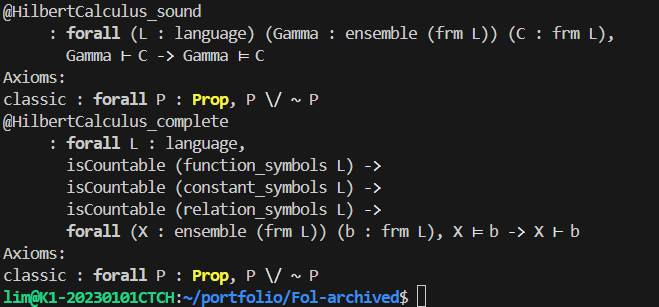
\includegraphics[width=1.0\linewidth]{OUTPUT.png}
                \caption{The result from the script.}
            \end{figure}
        }
    \end{minipage}

\end{frame}

% [script] 이어서 제 연구의 기여를 말씀드리겠습니다. 제 일차논리의 Coq 임베딩이 수학 프레임워크로써 기능할 수 있도록, 저는 등호가 있는 일차논리에 대한 메타정리를 전개하였습니다. 또한, embedded된 \Gamma로부터 embedded된 \phi가 증명될 필요충분조건이 \Gamma로부터 \phi가 증명된다는 것임을 보이는 것은 어느 선행 연구에서도 보이지 않았습니다. 두 번째로 언급한 선행 연구가 이것을 보이지 못해서 side condition을 만들었고, 마지막으로 언급한 선행 연구가 이것을 보이지 못해서 Henkin constant를 도입하지 않고 우회하여 증명하였습니다. 또한 제 가산 완전성 정리는 그 유명한 Enderton의 수리논리학 책에서 인용한 것이고 따라서 정통성이 있다고 할 수 있습니다. 게다가 자연 연역에 대한 연구가 상대적으로 많은데 따라서 힐베르트 계산을 형식화한 제 연구가 더 가치 있다고 말할 수 있습니다.
\begin{frame}{Conclusion}

    \textbf{The Contributions.}

    \begin{itemize}
        \item The fact that, for any set $\Gamma$ of $L$-formulae and any $L$-formula $\varphi$, \[ \embed{\Gamma} \vdash \embed{\varphi} \leftrightarrow \Gamma \vdash \varphi , \] had not been formalised in any former studies.
        \item My formal proof of the Countable Completeness Theorem closely follows the approach presented in Enderton's mathematical text, ensuring its fidelity to orthodox methodology.
        \item While there are many studies that formalise natural deduction, Hilbert calculi have received comparatively less attention. This makes my formalisation a significant contribution.
    \end{itemize}

\end{frame}

% [script] 마지막으로, 향후 연구 계획을 말씀드리겠습니다. 먼저, 수학 프레임워크로써 기능하는 실질적인 예를 찾을 것입니다. 후보로는 페아노 산술과 체르멜로-프렝켈 집합론을 염두에 두고 있습니다. 이 두 체계가 모두 공리꼴을 다루므로, 메타변수를 다루는 도구를 개발할 것입니다. 또한, 가산 일차 언어에 대한 완전성 정리를 형식 증명하였는데, 기수가 알레프 널보다 더 큰 일차 언어에 대한 완전성 정리도 형식 증명할 것입니다.
\begin{frame}{Conclusion}

    \textbf{Future Work.}

    \begin{itemize}
        \item The practical applicability of the framework such as $\mathsf{PA}$ and $\mathsf{ZF}$ will be explored.
        \item Since both systems have axiom schemata, a tool will be made for handling meta-variables.
        \item The Completeness Theorem for first-order languages with cardinalities greater than $\aleph_0$ will be formally proved as well.
    \end{itemize}

\end{frame}

% [script] 이상으로 발표를 마치겠습니다. 들어주셔서 감사합니다.
\begin{frame}
    \begin{center}
        \textit{\huge Thank you for listening!}
    \end{center}
    \begin{center}
        \begin{minipage}{0.77\textwidth}
            \begin{description}
                \item[{E-mail:}] \texttt{gijungdduk@naver.com}
                \item[{GitHub:}] \texttt{github.com/KiJeong-Lim/Fol-archived}
            \end{description}
        \end{minipage}
    \end{center}
\end{frame}

\end{document}
